\chapter{Intro to virus}
\label{cha:6}
%\documentclass[10pt]{article}\

%%%%%%%%%%%%%%%%%%%%%%%%%%%%%%%%%%%%%%%%%%%%%%%%%%%%%%%%%%
%%%%%			Introduction Chapter 6			%%%%%%
%%%%%												%%%%%%
%%%%%												%%%%%%
%%%%%%%%%%%%%%%%%%%%%%%%%%%%%%%%%%%%%%%%%%%%%%%%%%%%%%%%%%


\section{tekst}

In this section we are going to elaborate how we are going to model a Flipit game with multiple resources and a virus that propagates and infects the resources. We come up with a formula for the normal FlipIt and then reform it to a FlipIt game with a virus.

\subsection{FlipIt with a virus}
In the previous version the FlipIt game is already been explained. In this section we will introduce the virus propagation. An attacker will drop a virus on one of the resources that is available. The virus will then spread itself to the neighbour resources. The attacker will only gain control over the whole network, in general the game, when it has infected a certain amount of resources. We will call this amount for now ''d''. If we want to measure how many time it takes for the virus to infect ''d'' resources, we have to calculate the shortest path to the ''d'' th node.  If we know how much time it takes to control ''d'' resources, we can model a normal FlipIt game but with a delay. The model will not be completely a FlipIt game with a delay, because if the delay is bigger than the period of the attacker, the attacker will gain no control. If it would be with the delay the attacker would gain control after the defender flipt again. \todo{laten zien met een figuur}. In the next section we are going to describe what the setting of the game is.

\subsection{chap}
The setting of the game that we are going to play is one with multiple resources. When the defender flips it will always flip all the resources. The attacker will flip the node in the graph that can infect all the nodes in the shortest time possible. The attacker will gain the control over the resources when all the resources are infected. So ''d'' will be the shortest path to the furthest node. We will model ''d'' in time units. \todo{moet misschien niet ? }.
\begin{figure}[hbtp]
\caption{Difference in a FlipIt game between delay caused by a virus and a delay for the Attacker}
\centering
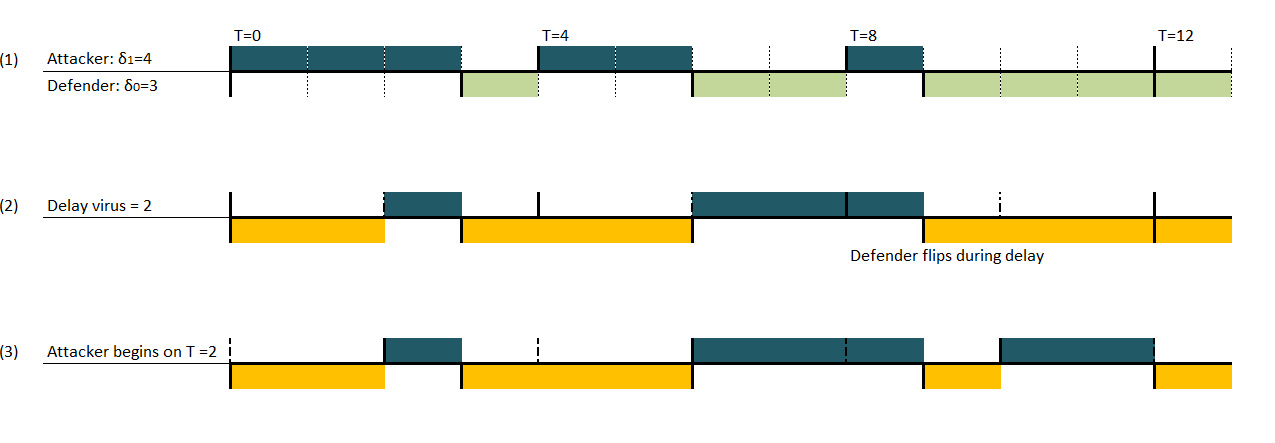
\includegraphics[scale=0.3]{Images/diffVirusDelay.jpg}
\end{figure}

If \textit{i} is an Irrational number:
$ i \neq \dfrac{a}{b}$ with $b \in Z, a \in N$
Because we cannot write \textit{i} in a fraction, this means that we won't have a cycle. If we would have a cycle that means that we do have a number that divides \textit{i}. If we don't have a cycle it goes on forever. Meaning that it goes on to infinity. This also means that no number will be repeated two times. If it does that means that their is repetition, meaning again that their is a cycle. We can conclude that if we have no cycle and no number will be repeated twice, that it will enumerate every number between 0 and the biggest interval. \todo{interval definieren}
Even though time is continious, irrational numbers are not considered. We kunnen continue tijd voldoende dicht benaderen door enkel rationele getallen in beschouwing te nemen. Vlakbij elk Irrationaal getal ligt immers een Rationaal getal.

A $\delta$ that is irrational will have no cycle. 

\subsection{define formula}
\begin{equation}\label{first}
n = \delta_{1} mod \delta_{0}
\end{equation}

\begin{equation}\label{first}
\Delta A = [( \delta_{0} - n + 1 ) * \delta_{1}] mod \delta_{1}
\end{equation}

\begin{equation}\label{first}
\sum_{i=0}^{\delta_{1}} \lbrace [( \delta_{0} - i + 1 ) * \delta_{1}] mod \delta_{1} \rbrace
\end{equation}
\todo{formule met i nakijken}

%\begin{equation}
%\Re{z} =\frac{n\pi \dfrac{\theta +\psi}{2}}{
%\left(\dfrac{\theta +\psi}{2}\right)^2 + \left( \dfrac{1}{2}
%\log \left\lvert\dfrac{B}{A}\right\rvert\right)^2}.
%\end{equation}
%
%\begin{equation}
%\boxed{\eta \leq C(\delta(\eta) +\Lambda_M(0,\delta))}
%\end{equation}
%
%\begin{equation}\label{first}
%a=b+c
%\end{equation}
%
%\begin{subequations}\label{grp}
%\begin{align}
%a&=b+c\label{second}\\
%d&=e+f+g\label{third}\\
%h&=i+j\label{fourth}
%\end{align}
%\end{subequations}



%%% Local Variables: 
%%% mode: latex
%%% TeX-master: "thesis"
%%% End: 


